% !TEX root = main.tex
\section{Implementation of a Dataflow Library in QL for SSA-dIMP}

In this section, we describe an implementation of the algorithm schema described in the
last section.
The implementation is written in QL.
As part of the project, we implemented a library and a database scheme for SSA-dIMP.
On top of that, the dataflow algorithm is implemented.

The implementation itself is very easy, but the structure follows the
dataflow library used for Java.
It is useful, because it demonstrates how to bridge the gap between
the theoretical description of the algorithm with the soundness proof
as in \autoref{sec:df-theory} and the actual implementation of dataflow
in QL for languages like Java.
However, all the features that complicate the dataflow library for Java have been 
omitted.
The most complicated feature is that the Java dataflow library supports tracking 
flow through fields, i.e.\ if a variable that received data from a source 
is assigned to a field in an object, and a sink later reads from that field,
dataflow is detected.
Furthermore, the Java dataflow library is an interprocedural analysis.
Thus, the implementation has to be done very carefully to exhibit good
performance on large projects.

\subsection{The Database Scheme}
The database scheme is given in full in the \hyperref[lst:dbscheme]{appendix}.
The database contains a representation the abstract syntax tree (AST) of the program.
For each arithmetic expression, its unique ID, its kind
(i.e.\ integer literal, addition, multiplication, \ldots) 
and the ID of the type of the expression are saved.
Furthermore, another table contains the parent-child relation for arithmetic 
expressions - every tuple there contains the ID of an expression parent 
(either an arithmetic expression, a Boolean expression or a statement),
the ID of the child arithmetic expression and the index.
For example the addition $a_0 + a_1$ has as first child the ID of the expression 
$a_0$, and as second child the ID of the expressions $a_1$.
The order of these is an implementation detail of the database scheme in combination
with the extractor (that writes the database) and the standard library 
(that is built on top of the database scheme).

A similar database layout is employed for statements and Boolean expressions.
Expressions like literals have another relation that tracks the actual value of the
literal, variable reads have a relation that tracks the variable that is read,
variable assignments have a relation that tracks the variable that is assigned to, etc.

The database scheme is quite close how a compiler would model an AST for SSA-dIMP.
It is certainly inspired by the QL database scheme for Java.
There is one crucial difference though - in SSA-dIMP the AST is already in SSA form,
and we assume that sets $\Gamma, \Delta$ exist to prove that.
Programs in Java are not in SSA form.
Thus, as part of the QL library for Java, there exists an SSA construction algorithm
that synthesizes an SSA form.
As this is computed on the fly, it is not represented in the database scheme.

Essentially, this makes the implementation of the library for SSA-dIMP easier,
as we dont have to deal with the SSA construction.
Constructing the SSA form of a program is a well-researched problem in compiler
construction, so we feel confident that assuming the existence of an SSA form 
of the program does not lower the value of this project.

\subsection{The Standard Library}
The standard library for SSA-dIMP is implemented in the file \hyperref[lst:library]{library.qll}.

The standard library offers an object-oriented interface on top of the relational
database scheme.
Again, this interface is inspired by the corresponding library for Java.

The library offers interfaces for arithmetic expressions, and each kind of expression
has a sub-class available in the standard library.
As the QL language requires toString predicates on all classes,
the standard library also provides pretty-printing for the entire AST.

Furthermore, for example the class representing a Variable offers access to the
reads of that variable (phi nodes and variable access expressions), as well
as access to the statements that assign to this variable.
Also, the parent-child relation is exposed, and used to implement named helper predicates.
For example, for an if statement, the child branches are exposed as \texttt{getThenBranch()}
and \texttt{getElseBranch()}.
This hides the implementation detail that the then branch is the first child of the
if statement, and the else branch the second.

\subsection{The Dataflow Algorithm}
As the algorithm in \autoref{sec:df-theory} computes a type for all expressions and statements in the program,
it implicitly runs on the AST.
The algorithm in practice is given in \hyperref[lst:dataflow]{dataflow.qll}.

\subsubsection*{Step 1 - The Dataflow Graph}
TODO change
Typing an entire AST to detect dataflow is quite inefficient, so the algorithm
runs on a different graph, the \emph{dataflow graph}.
It is a datastructure that makes it easy to compute a typing derivation as needed to
detect dataflow.
The node set of the dataflow graph is a subset of the node set of the AST.

The dataflow graph keeps track of which expressions and statements potentially get data from a source.
The node set of the dataflow graph contains all AST nodes of the following form:
\begin{itemize}
    \item all expressions of kind variable access and source
    \item statements of kinds assign and sink
    \item all $\varphi$-nodes
\end{itemize}

All of these nodes then get tagged in step 2 with a label.
For the expressions, this directly corresponds to the type in the refined type system
as presented in~\autoref{sec:df-theory}.
For assign statements and $\varphi$-nodes, this label corresponds to the type of 
the variable that is defined, and for sinks the label corresponds to the type
of the expression that is passed to the sink.

We can restrict the node set to these expression kinds, as all other expression kinds
are always tagged with $\lclean$.
The only relevant statements for dataflow are assign and sink, as all DF rules for the 
other statements just pass through labels, but don't define new labels.
Thus, the node set contains  exactly the relevant elements of the AST that are involved in determining
if a program has dataflow or not.

Building the dataflow graph is done by defining the \texttt{flowStep} relation on the node set.
It contains the tuple $(\textit{node1}, \textit{node2})$ if the label of \textit{node2} is directly affected
by the label of \textit{node1}.
Thus, the edges of the dataflow graph indicate along which paths dataflow tracking marker propagate
through the program.

For example, if an expression node has type $\ltracked$,
all downstream expression nodes on a path from the first expression node 
have type either $\ltracked$ or $\lunknown$ (and not $\lclean$).
We combine this propagation information with the location of the sinks and sources 
to detect potential dataflow.

The rules to construct the dataflow graph are as follows:

By looking at the typing rule for statements, we see that only assign and sink statements
use the tracking marker assigned to the arithmetic expression used in that statement.
Thus, there is an edge from the right-hand side of an assignment (the expression) 
to the node for the assign statement, as well as from the operand from the sink 
to the node for the sink statement.

The other cases in \texttt{flowStep} deal with variable definitions.
There is an edge from every variable definition (which is either a $\varphi$-node or 
an assign statement) to all users of that variable, i.e. to all expressions of kind
variable access, as well as all $\varphi$-nodes that have the variable as input.
Formulated differently, there is an edge from a variable definition to all of its uses.

There are no incoming edges for source expressions, as the result of a source expression
is always tainted.

We now show the dataflow graph for the example program (\autoref{fig:ssa-dimp-example}).
Node types (expression, $\varphi$ or statement) are not indicated, but are obvious from context.
Furthermore, the place of the variable accesses in the AST is only indicated when it is 
not clear from the context.
However, as every node in the dataflow graph is also a node in the AST, all the variable accesses
of one variable are different nodes in the dataflow graph.

TODO line numbers (maybe)
TODO QL dump of graph

\begin{figure}[h]
    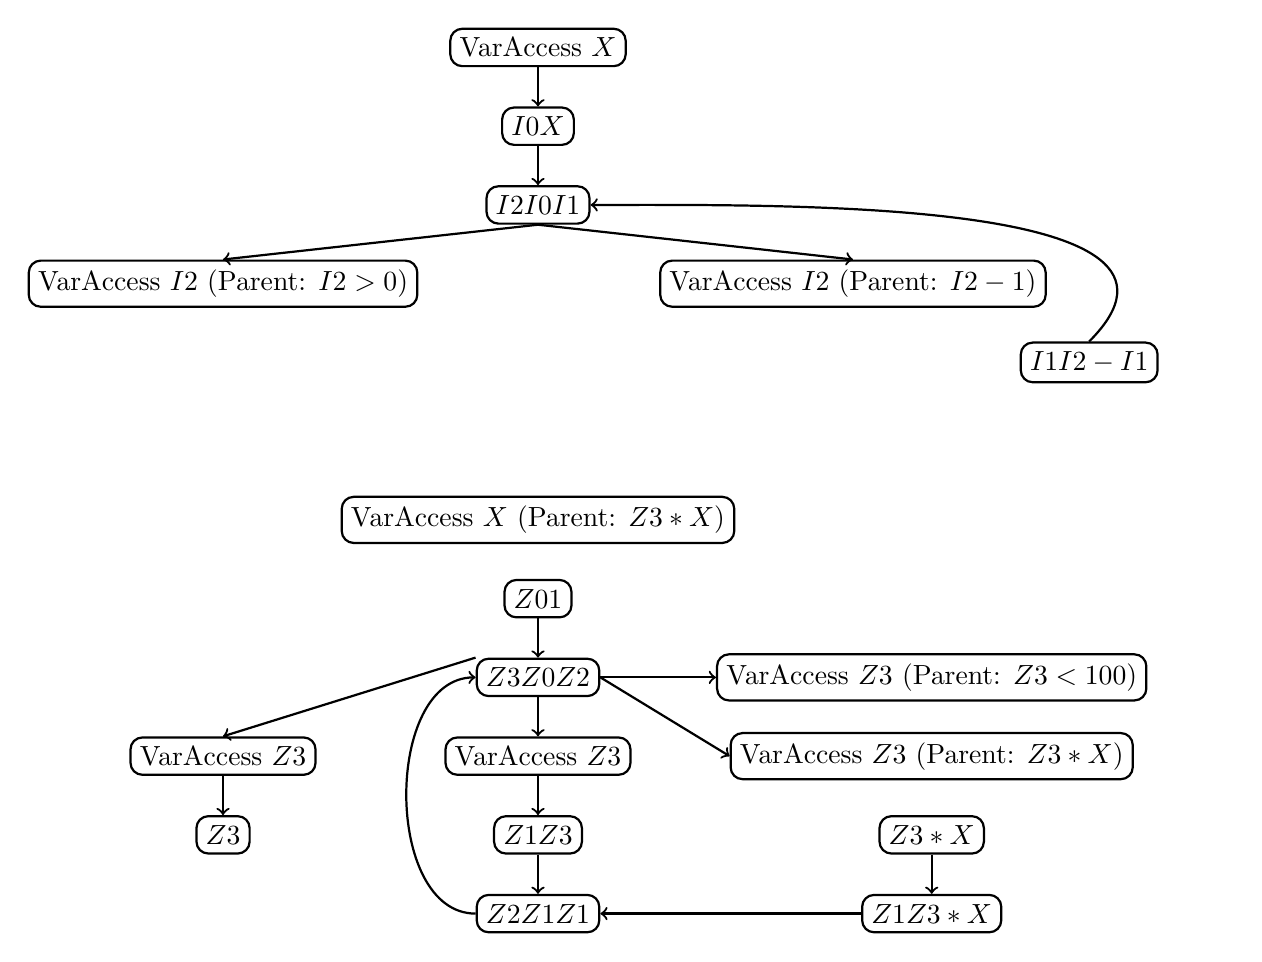
\begin{tikzpicture}[roundnode/.style={rectangle,rounded corners=1ex,draw=black!100,thick},->,thick]
        \node[roundnode] (storez0) at(0, 0) {$\storecmd{Z0}{1}$};
        \node[roundnode] (phiz3) at (0, -1) {$\phistore{Z3}{Z0}{Z2}$};
        \node[roundnode] (varaccessbool) at (5, -1) {VarAccess $Z3$ (Parent: $Z3 < 100$)};
        \node[roundnode] (multvaraccess) at (5, -2) {VarAccess $Z3$ (Parent: $Z3 * X$)};
        \node[roundnode] (multvaraccess2) at (0, 1) {VarAccess $X$ (Parent: $Z3 * X$)};
        \node[roundnode] (source) at (5, -3) {$\source{Z3 * X}$};
        \node[roundnode] (storemult) at (5, -4) {$\storecmd{Z1}{\source{Z3 * X}}$};
        \node[roundnode] (varaccessz4) at (0, -2) {VarAccess $Z3$};
        \node[roundnode] (storez1) at (0, -3) {$\storecmd{Z1}{Z3}$};
        \node[roundnode] (phiz2) at (0, -4) {$\phistore{Z2}{Z1}{Z1}$};
        \node[roundnode] (varaccessz42) at (-4, -2) {VarAccess $Z3$};
        \node[roundnode] (sink) at (-4, -3) {$\sink{Z3}$};
        \draw (storez0.south) -- (phiz3.north);
        \draw (phiz3.east) -- (varaccessbool.west);
        \draw (phiz3.east) -- (multvaraccess.west);
        \draw (storemult.west) -- (phiz2.east);
        \draw (phiz3.south) -- (varaccessz4.north);
        \draw (varaccessz4.south) -- (storez1.north);
        \draw (storez1.south) -- (phiz2.north);
        \draw (phiz2.west) to [out=180,in=180] (phiz3.west);
        \draw (phiz3.north west) -- (varaccessz42.north);
        \draw (varaccessz42.south) -- (sink.north);
        \draw (source.south) -- (storemult.north);
        \node[roundnode] (ivarx) at (0, 7) {VarAccess $X$};
        \node[roundnode] (i0getsx) at (0, 6) {$\storecmd{I0}{X}$};
        \node[roundnode] (phii2) at (0, 5) {$\phistore{I2}{I0}{I1}$};
        \node[roundnode] (readi21) at (-4, 4) {VarAccess $I2$ (Parent: $I2 > 0$)};
        \node[roundnode] (readi22) at (4, 4) {VarAccess $I2$ (Parent: $I2 - 1$)};
        \node[roundnode] (writei1) at (7, 3) {$\storecmd{I1}{I2 - I1}$};
        \draw (ivarx.south) -- (i0getsx.north);
        \draw (i0getsx.south) -- (phii2.north);
        \draw (phii2.south) -- (readi21.north);
        \draw (phii2.south) -- (readi22.north);
        \draw (writei1.north) to [in=0] (phii2.east);
    \end{tikzpicture}
    
    \caption{The dataflow graph for the example program}
\end{figure}

\subsubsection*{Step 2 - Labeling Nodes}
As second step, the algorithm computes a labelling of the nodes of the dataflow graph.
This labelling can be used to easily determine if a program is safe to execute or not.
Furthermore, this labelling can be used to construct a typing derivation (by the DF-rules)
of the program.
Note that in the dataflow graph, all $\varphi$-nodes have indegree 2, whereas all
non-$\varphi$-nodes have indegree 0 or 1.

TODO explain this much better

First, the predicate \texttt{nodeLabelCand} computes a set of candidate labels 
for each node in the dataflow graph:
The labelling starts at nodes in the graph without incoming edges.
These can be labelled with $\ltracked$ (if the node is an expression node of kind source),
or with $\lclean$ otherwise (the node represents a read of a variable initialized outside
of the program, an variable assignment of an expression that is marked as clean).

All $\varphi$-nodes are marked with $\lunknown$.
If all incoming edges to a $\varphi$-node agree on a label, this label is then
also applied to the $\varphi$-node.

All non-$\varphi$-nodes that have an incoming edge inherit all tracking markers from
the previous node.

As second step, the predicate \texttt{nodeLabel} computes the best label for each node 
among all candidate labels:
If a node is both marked with $\lclean$ and $\lunknown$ or both with $\ltracked$
and $\lunknown$, the more specific marking is chosen.
By construction, the algorithm never marks a node with both $\lclean$ and $\ltracked$,
as nodes without incoming edges only get a single label, and $\varphi$-nodes only 
propagate a label if all immediate predecessors have the same label.

With that information, the dataflow query can report all nodes of type sink.
If any of them has the label $\lunknown$ or $\ltracked$, then we know that the sink
is unsafe, because it (potentially) reads from a source.

\subsubsection*{Step 3 - Building  a Typing Derivation}
TODO change name of the section, not as part of the algorithm itself
used to prove correctness/certificate

TODO include non-empty deltas for commands for SSA-dIMP program

While the information in step 2 is enough to detect unsafe sinks,
which is needed to apply~\autoref{thm:soundness-df},
we can use the computed labels to build a typing derivation for the whole program
using the DF rules.

Remember that the DF rules are non-deterministic only in the rule \textsc{DF-While},
so the process of building a typing derivation is straight-forward, except for while loops.

The initial map $\Gamma$ is given by mapping all variables that are defined in 
the initial store to $\lclean$.

The typing rules for booleans are satisfied by the assumption that the program 
is well-typed with respect to the SSA rules.

Expressions that have a label assigned to them in \texttt{nodeLabel} get that label.
All other expressions are typed with $\lclean$.
Using this, we immediately get the map $\Delta$ for the rule $\textsc{DF-Assign}$.

For all other statements, we compute the derivation tree recursively,
following the rules.
At any place where the rule \textsc{DF-$\varphi$} is used, the map $\Delta$ 
is determined by the labels of the respective $\varphi$-nodes in $\texttt{nodeLabel}$.
Using this, we can compute the map $\Delta_1$ used in \textsc{DF-While} using the
standard recursive procedure, as $\Gamma \union \Delta$ is now defined.
This alleviates the need to guess for this rule.
All other rules can directly be used to infer the type derivation.

\subsubsection*{On the Relation of the Algorithm to the DF Typing Rules}
As explained above, this algorithm runs already on SSA-dIMP, not dIMP.
Thus, we assume that the SSA construction already took place.
As conjectured in~\autoref{con:dimp-to-ssa}, any dIMP program can be transformed into an equivalent
SSA-dIMP program.
This transformation also (implicitly) takes care of the concrete semantics of e.g.\ 
while and if statements - the dataflow algorithm only expects correctly placed $\varphi$-nodes,
and does not depend on the semantics of the individual statements.

If, for example, a repeat-until loop construct would be added to the language,
SSA-dIMP could be easily extended with that loop construct by adding a new statement 
kind to the database and implementing the library.
However, the dataflow algorithm itself would work without any changes, assuming that
the $\varphi$-node placement is correct.
This is very different from the algorithm schema with the DF rules that depends intimately on the 
typing schema, and this might be puzzling at first.
This apparent contradiction can be resolved by seeing that the DF typing 
rules serve two purposes - first, they are a refinement of the SSA typing rules,
and second, they describe an approximation on where dataflow occurs.

As the dataflow algorithm as presented here assumes that the program is already in 
SSA form, it can do substantially less than what is described in the DF rules.
In particular, it only has to worry about the introduction of flow in expressions,
and the propagation of the tracked marking to variable stores and to sinks.
Thus, it can safely skip the entire part of the rules that deal with scoping.

%The tracked marker for variable reads is fully determined by the type context,
%which we do not explicitly compute.
%In the implicit formulation, a variable access gets the tracking marker of its definition,
%which is, because the program is in SSA form, unique.
%If the variable definition is an assign statement, this follows immediately from the
%\textsc{DF-Assign} rule - the variable is tagged with the marker of the expression.
%Thus, we have an edge from the expression node to that of the 
%If the variable is defined in a $\varphi$-node, we have compute the least upper bound of 
%both variables that make up the $\varphi$-node.
%This is implicit in the algorithm, as the $\varphi$-node will have an incoming edge if 
%at least one of the variables is marked with $\ltracked$ or $\lunknown$.
%However, in both cases, we have flow from a variable definition (either an assign
%statement or a $\varphi$-node) to a variable read (either a VarAccess expression, 
%or another $\varphi$-node).

\subsubsection*{Simplification of the Algorithm}
In practice, we can optimize the algorithm even more.
This is done by reducing the lattice and only keeping $\lclean$ and $\lunknown$.
Then, we do not need an explicit node label anymore, a predicate can now
keep track of all nodes that are marked with $\lunknown$ (the only relevant nodes 
for dataflow).
Furthermore, we can restrict ourselves to connected components of the dataflow graph
that start in a source node.
All other parts of the dataflow graph can be discarded, as they do not contribute 
to detecting dataflow.
In fact, nodes in this restricted dataflow are marked with $\lunknown$ if there
exists a path from a source to the node.
Especially, this means a program is (potentially) dangerous if there exists a path
from a node of type source to a node of type sink.
This problem can be solved very efficiently.
The QL implementation can be found in the predicate \texttt{reaches},
that computes all reachable nodes from a sink.
If this predicate contains any sink nodes, the program is deemed unsafe.

This algorithm marks the same programs as unsafe as the previously proposed implementation,
but it does obviously not include the distinction between $\lunknown$ and $\ltracked$.
The theoretical groundwork as laid out in~\autoref{sec:df-theory} can be applied,
but using a two-point lattice with elements $\lunknown$ and $\lclean$ instead.
The soundness proof goes through essentially unchanged.
Thus, a typing derivation using the DF rules (with the simplified lattice) 
can be reconstructed, as explained above.

The example can also be adapted: In the example dataflow graph, one can easily
see that there is a path from the source to the sink, so that program is unsafe.

\subsection{The Query}
The query actually implementing the user-facing analysis is given in \hyperref[lst:query]{query.ql}.
It is very simple, it outputs a list of sinks if their label is either unknown or tracked.
If the list is empty, the program is safe and it is guaranteed by~\autoref{thm:soundness-df}
that the program has no dataflow.
If the list is not empty, no assertion about the program correctness can be given.
